\documentclass[12pt]{article}
\usepackage[utf8]{inputenc}
\usepackage{multicol}
\usepackage{fancyhdr}
\usepackage{gensymb}
\usepackage{graphicx}
\usepackage{listings}
\usepackage{color}
\usepackage[margin=1in]{geometry}
\usepackage{tcolorbox}

\lstset{frame=tb,
  language=Matlab,
  aboveskip=3mm,
  belowskip=3mm,
  showstringspaces=false,
  columns=flexible,
  basicstyle={\small\ttfamily},
  numbers=none,
  numberstyle=\tiny\color{gray},
  keywordstyle=\color{blue},
  commentstyle=\color{dkgreen},
  stringstyle=\color{mauve},
  breaklines=true,
  breakatwhitespace=true,
  tabsize=3
}
\definecolor{dkgreen}{rgb}{0,0.6,0}
\definecolor{gray}{rgb}{0.5,0.5,0.5}
\definecolor{mauve}{rgb}{0.58,0,0.82}

\begin{document}

\begin{titlepage}
    \begin{center}
        \vspace*{1cm}
            
        \LARGE
        \textbf{PIV Analysis: Starting Vortex}
            
        \vspace{0.5cm}
        \Large
        Aerodynamics and Propulsion
Laboratory 
            
        \vspace{1.5cm}
        \large
        \textbf{Section 2}\\
        \normalsize\vspace{15 pt}
        Tyler Cascalho Cox\\
        \vfill
            
            
        \vspace{0.8cm}
            
            
        \Large
        Iowa State University\\
        Undergraduate Aerospace Engineering
        
            
    \end{center}
\end{titlepage}


\pagestyle{fancy}
\fancyhead[LE,RO]{\normalsize Section 2}
\fancyhead[RE,LO]{\normalsize PIV Analysis: Starting Vortex}
\fancyfoot[CE,CO]{\leftmark}
\fancyfoot[LE,RO]{\thepage}


\section*{Abstract}
In this report PIV analysis is used to measure the vorticity of the starting vortex of a NACA 63-212 airfoil emerged in water. The data obtained from this experiment is then used to determine the effects of viscosity on the starting vortex over time.
\newline
\section*{Variables and Symbols}
\(u\) - Flow Velocity \(\left(\frac{\mbox{m}}{\mbox{s}}\right)\)\newline\newline
\(V\) - Vorticity \(\left(\frac{1}{{\mbox{s}}}\right)\) \newline\newline



\newline
\newpage
\tableofcontents
\label{sec:Abstract}
\addcontentsline{toc}{section}{\nameref{\hspace{10 pt} Abstract}}
\newpage

\section{Introduction}
In this experiment, the main focus is the formation and decay of the starting vortex. To do this a PIV analysis system will be used. PIV analysis is ideal for studying the starting vortex since it gives the velocity field of the fluid which can then be used to find the vorticity at any given moment.  

\newpage
\section{Theory}
\subsection{PIV Measurement}
    \begin{figure}[h]
    \includegraphics[width=12 cm]{pic1.PNG}
    \centering
    \caption{Schematic of experimental setup for starting vortex PIV measurement}
    \end{figure}
    In PIV a fine grained reflective material is added to the water to act as a tracer. A laser is then shot through a cylindrical lens making a laser sheet which is then aimed at the test section. A camera is placed perpendicular to the plane so that it can capture the entire plane eliminated by the laser. While moving the airfoil through the test section the camera then takes a plethora of photo pairs which are then used to determine the velocity of the fluid by detecting how far, in pixels, the tracers moved between shots. A calibration photo is then used to then convert that distance from pixels to meters.
\subsection{Starting vortex}
The starting vortex is the vortex that is formed next to the trailing edge of an airfoil as it is accelerated from rest. Once it leaves the airfoil it remains stationary in the flow and decays due to viscous interactions in the flow.


\newpage
\section{Experimental Setup}
\subsection{General Description}
Figure 1, shows the schematic of the experimental setup for this study. An airfoil (NACA 63-212) is mounted inside a water tank attached to a rail allowing the airfoil to be manually traversed inside the tank. The tank water is seeded with hollow glass micro-spheres (\(\sim\)25 \(\mu\)m, density of 1.1 \(\mbox{g}/\mbox{cm}^3\)). The illumination is provided with a continuous-wave laser with 405 nm wavelength. The laser beam is converted to a thin sheet using a cylindrical lens that is then passed through the tank, perpendicular to the airfoil. The scattered light from the seed particles is imaged onto a CMOS camera. After imaging the photos are then MATLAB's PIVlab app, which is used to process the images. The vorticity data is for each image pair is extracted into a text file and then plotted.
    \begin{figure}[h]
    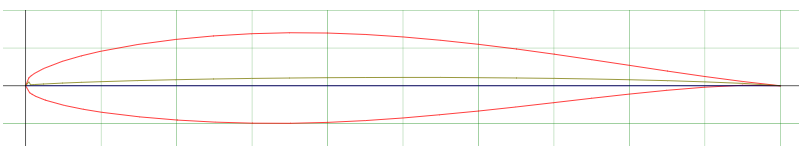
\includegraphics[width=14 cm]{airfoil.PNG}
    \centering
    \caption{NACA 63-212 Airfoil}
    \end{figure}


\subsection{Case Study}
The lab was at NTP during the experiment
\begin{itemize}
    \item \(P_{ntp} = 1 \hspace{3 pt}\mbox{atm}\)
    \item  \(\rho_{ntp} = 1.225  \hspace{3 pt}\frac{\mbox{kg}}{{\mbox{m}}^3}\)
    \item \(T_{ntp} = 20 \hspace{3 pt}\degree\mbox{C}\)
\end{itemize}

\newpage
\section{Results}
\subsection{Resolution Calculation}

    
Image base resolution is \(484 \times 364\) Pixels
\newline
Analysis was done with a min window size of 16 which means that the resolution of the analysis is:

\[\frac{484}{16} \times \frac{364}{16} \approx 30 \times 23 \hspace{2 pt} \mbox{Pixels}\]
\subsection{Velocity Distribution for Image 100}
    \begin{figure}[h]
    \includegraphics[width=16 cm]{v1.PNG}
    \centering
    \caption{Velocity Distribution for Image 100}
    \end{figure}
    
    \newpage
    \subsection{Velocity Distribution for Image 120}
    \begin{figure}[h]
    \includegraphics[width=16 cm]{v2.PNG}
    \centering
    \caption{Velocity Distribution for Image 120}
    \end{figure}
    
    \newpage
    \subsection{Velocity Distribution for Image 175}
    \begin{figure}[h]
    \includegraphics[width=16 cm]{v3.PNG}
    \centering
    \caption{Velocity Distribution for Image 175}
    \end{figure}
    
    \newpage
    \subsection{Velocity Distribution for Image 275}
    \begin{figure}[h]
    \includegraphics[width=16 cm]{v4.PNG}
    \centering
    \caption{Velocity Distribution for Image 275}
    \end{figure}
    
    \newpage
    \subsection{Velocity Distribution for Image 350}
    \begin{figure}[h]
    \includegraphics[width=16 cm]{v5.PNG}
    \centering
    \caption{Velocity Distribution for Image 350}
    \end{figure}
        
    \newpage
    \subsection{Velocity Distribution for Image 430}
    \begin{figure}[h]
    \includegraphics[width=16 cm]{v6.PNG}
    \centering
    \caption{Velocity Distribution for Image 430}
    \end{figure}
        
    \newpage
    \subsection{Velocity Distribution for Image 530}
    \begin{figure}[h]
    \includegraphics[width=16 cm]{v7.PNG}
    \centering
    \caption{Velocity Distribution for Image 530}
    \end{figure}
    
    \newpage
    \subsection{Vorticity Distribution for Image 100}
    \begin{figure}[h]
    \includegraphics[width=16 cm]{v1.1.jpg}
    \centering
    \caption{Vorticity Distribution for Image 100}
    \end{figure}
    
    \newpage
    \subsection{Vorticity Distribution for Image 120}
    \begin{figure}[h]
    \includegraphics[width=16 cm]{v2.1.jpg}
    \centering
    \caption{Vorticity Distribution for Image 120}
    \end{figure}
    
    \newpage
    \subsection{Vorticity Distribution for Image 175}
    \begin{figure}[h]
    \includegraphics[width=16 cm]{v3.1.jpg}
    \centering
    \caption{Vorticity Distribution for Image 175}
    \end{figure}
    
    \newpage
    \subsection{Vorticity Distribution for Image 275}
    \begin{figure}[h]
    \includegraphics[width=16 cm]{v4.1.jpg}
    \centering
    \caption{Vorticity Distribution for Image 275}
    \end{figure}
    
    \newpage
    \subsection{Vorticity Distribution for Image 350}
    \begin{figure}[h]
    \includegraphics[width=16 cm]{v5.1.jpg}
    \centering
    \caption{Vorticity Distribution for Image 350}
    \end{figure}
        
    \newpage
    \subsection{Vorticity Distribution for Image 430}
    \begin{figure}[h]
    \includegraphics[width=16 cm]{v6.1.jpg}
    \centering
    \caption{Vorticity Distribution for Image 430}
    \end{figure}
        
    \newpage
    \subsection{Vorticity Distribution for Image 530}
    \begin{figure}[h]
    \includegraphics[width=16 cm]{v7.1.jpg}
    \centering
    \caption{Vorticity Distribution for Image 530}
    \end{figure}


    \newpage
    \subsection{Max Vorticity Distribution vs Time}
    \begin{figure}[h]
    \includegraphics[width=16 cm]{vt.jpg}
    \centering
    \caption{Max Vorticity Distribution vs Time}
    \end{figure}

\subsection{General Discussion of Results and of Error}
When processing the data vectors that seemed out of place were removed. This was determined by looking around any given velocity vector and seeing if the velocity vectors around it were not demonstrably smaller or larger than it. As discussed in the Theory it can be seen that the max vorticity of the starting vortex decays with time due to the viscous nature of the fluid, which can be clearly seen in Figure 17.


\newpage
\section{Conclusion}
The starting vortex plays an important part in lift and it can be effectively analysed using a PIV system. More importantly PIV analysis is an extremely powerful tool allowing one to measure the velocity field in a whole plane instead of just at a point unlike a pressure tap. This is highly advantageous since it gives the bigger picture of the dynamics for the flow, opening up new avenues for analysis.
\newline
\newline
For future study, it would be interesting to find the correlation between max shedding vorticity and airfoil speed, airfoil shape, different fluid viscosity's, or angle of attack. The proposed study would use a setup similar to Figure 1 and then choose one of the aforementioned variables to vary (i.e. airfoil shape) and hold the rest constant. PIV would then be used to measure the max shedding vorticity of the starting frequency using the methods discussed in this report.



\newpage
\section{Work Cited}
Department of Aerospace Engineering. "Lab 12 Instructions". Lab handbook. Iowa State University. Ames, Iowa. 2020. Print.
\newline
\newpage
\setcounter{section}{0}
\def\thesection{\Alph{section}}
\section{Appendix of Data Tables}
    \begin{figure}[h]
    \includegraphics[width=14 cm]{maxV.PNG}
    \centering
    \caption{Max Vorticity Value of Starting Vortex in \(\frac{1}{\mbox{s}}\)}
    \end{figure}

    \begin{figure}[h]
    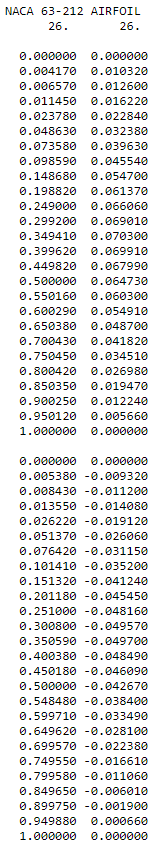
\includegraphics[width=2.5 cm]{dat.PNG}
    \centering
    \caption{NACA 63-212 airfoil data (Normalized to chamber)}
    \end{figure}

\newpage
\section{Appendix of Matlab Code}
\subsection{Code for Plots and Data Manipulation}
\begin{lstlisting}
%%
%Extract data
ft1 = load('DataAnalysis\1-1.txt');
ft2 = load('DataAnalysis\2-1.txt');
ft3 = load('DataAnalysis\3-1.txt');
ft4 = load('DataAnalysis\4-1.txt');
ft5 = load('DataAnalysis\5-1.txt');
ft6 = load('DataAnalysis\6-1.txt');
ft7 = load('DataAnalysis\7-1.txt');

%%
[m1, c1]=min(ft1(:,4));
[m2, c2]=min(ft2(:,4));
[m3, c3]=min(ft3(:,4));
[m4, c4]=min(ft4(:,4));
[m5, c5]=min(ft5(:,4));
[m6, c6]=min(ft6(:,4));
[m7, c7]=min(ft7(:,4));

figure(1)
plot(ft1(:,1)-ft1(c1,1),ft1(:,4))
xlabel("Distance on line [m]")
ylabel("Vorticity [1/s]")

figure(2)
plot(ft2(:,1)-ft2(c2,1),ft2(:,4))
xlabel("Distance on line [m]")
ylabel("Vorticity [1/s]")

figure(3)
plot(ft3(:,1)-ft3(c3,1),ft3(:,4))
xlabel("Distance on line [m]")
ylabel("Vorticity [1/s]")

figure(4)
plot(ft4(:,1)-ft4(c4,1),ft4(:,4))
xlabel("Distance on line [m]")
ylabel("Vorticity [1/s]")

figure(5)
plot(ft5(:,1)-ft5(c5,1),ft5(:,4))
xlabel("Distance on line [m]")
ylabel("Vorticity [1/s]")

figure(6)
plot(ft6(:,1)-ft6(c6,1),ft6(:,4))
xlabel("Distance on line [m]")
ylabel("Vorticity [1/s]")

figure(7)
plot(ft7(:,1)-ft7(c7,1),ft7(:,4))
xlabel("Distance on line [m]")
ylabel("Vorticity [1/s]")


mv = [m1 m2 m3 m4 m5 m6 m7];
t = ([100 120 175 275 350 430 530]-100)./100;

figure(8)
plot(t,mv)
xlabel("Time [s]")
ylabel("Vorticity [1/s]")


\end{lstlisting}



\end{document}
